\section{$d$-Cut}

\begin{frame}{$d$-Cut}
    \begin{block}{}
        A bipartition $(A,B)$ of $V(G)$ is a $d$-cut if and only if each vertex has at most $d$ neighbors across the cut.
    \end{block}
    
    
    \begin{figure}[!htb]
        \centering
        \onslide<2->
        \hspace{-0.4cm}
        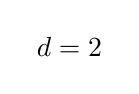
\begin{tikzpicture}[scale=1]
                %\draw[help lines] (-5,-5) grid (5,5);
                \node at (0,2) {$d=2$};
                \GraphInit[unit=3,vstyle=Simple]
                \SetVertexSimple[Shape=circle, FillColor=black, MinSize=2pt]
                \tikzset{VertexStyle/.append style = {inner sep = \inners, outer sep = \outers}}
                \SetVertexNoLabel
                \grCycle[RA=1.5, prefix=c]{4}
                \AddVertexColor{white}{c0,c1,c3}
                \AddVertexColor{black!50}{c2}
        \end{tikzpicture}
        \onslide<3->
        \hspace{1.4cm}
        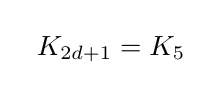
\begin{tikzpicture}[scale=1,rotate=90]
                %\draw[help lines] (-5,-5) grid (5,5);
                \GraphInit[unit=3,vstyle=Simple]
                \SetVertexSimple[Shape=circle, FillColor=black, MinSize=2pt]
                \onslide<6->{\node at (2.2,0) {$K_{2d+1} = K_5$};}
                \tikzset{VertexStyle/.append style = {inner sep = \inners, outer sep = \outers}}
                \SetVertexNoLabel
                \grComplete[RA=1.5,prefix=p]{5}
        \end{tikzpicture}
        \onslide<4->
        \hspace{1cm}
        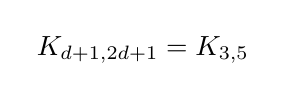
\begin{tikzpicture}[scale=1, rotate=-90]
                %\draw[help lines] (-5,-5) grid (5,5);
                \GraphInit[unit=3,vstyle=Simple]
                \SetVertexSimple[Shape=circle, FillColor=black, MinSize=2pt]
                \tikzset{VertexStyle/.append style = {inner sep = \inners, outer sep = \outers}}
                \SetVertexNoLabel
                \onslide<7->{\node at (-0.6,1) {$K_{d+1,2d+1} = K_{3,5}$};}
                \grCompleteBipartite[RA=0.8, RB = 0.7, RS=1.5]{3}{5}
        \end{tikzpicture}
    \end{figure}
    \onslide<5->
    \begin{block}{}
        A set $S \subseteq V(G)$ is \textit{monochromatic} if, in every $d$-cut $(A, B)$, it holds that $S \subseteq A$ or $S \subseteq B$.
    \end{block}
\end{frame}

\begin{frame}{Regular graphs are hard}
    \begin{theorem}
        \pname{$d$-Cut} on $(2d+2)$-regular graphs is $\NPH$.
    \end{theorem}
    \pause
    \begin{block}{\pname{3-Uniform Hypergraph Bicoloring}}
        \textit{Instance}: A hypergraph $\mathcal{H}$ with three vertices in each hyperedge.
        \textit{Question}: Can we 2-color $V(\mathcal{H})$ such that no hyperedge is monochromatic?
    \end{block}
    \pause
    \begin{block}{}
        Heavily inspired on the reduction given by:  \fullcite{chvatal_matching_cut}.
    \end{block}
\end{frame}

\begin{frame}{Monochromatic gadget: Spools}
    \begin{columns}[T]
        \begin{column}{0.44\textwidth}
        \begin{figure}[!htb]
            \centering
            \begin{tikzpicture}[scale=1]
                %\draw[help lines] (-5,-5) grid (5,5);
                \GraphInit[unit=3,vstyle=Simple]
                \SetVertexSimple[Shape=circle, FillColor=black, MinSize=1pt]
                \tikzset{VertexStyle/.append style = {inner sep = \inners, outer sep = \outers}}
                \SetVertexNoLabel
                \foreach \x in {0,1,2} {
                    \pgfmathtruncatemacro{\med}{(\x)*120 + 30}
                    \begin{scope}[rotate=-\med]
                        \draw (0,1.85) ellipse (1.6cm and 0.4cm);
                        \onslide<6>{\draw[thick, color=red] (0,1.45) -- (0,2.25);}
                    \end{scope}
                    \foreach \y in {0,1,2,3,4,5} {
                        \pgfmathtruncatemacro{\ang}{\x * 120 + \y * 24}
                        \Vertex[a=\ang, d=2.2]{i\x\y}
                    }
                    \foreach \y in {0,1,2} {
                        \pgfmathtruncatemacro{\ang}{\x * 120 + \y * 30 + 30}
                        \pgfmathsetmacro{\bla}{0.5 + mod(\y,2) *0.25}
                        \Vertex[a=\ang, d=\bla]{o\x\y}
                        \foreach \z in {0,1,2,3,4,5} {
                            \Edge(i\x\z)(o\x\y)
                        }
                    }
                }
                \onslide<2>{
                    \draw[thick,color=red] (-1.3,2.3) arc (50:-50:3);
                    \node[color=red] at (-2.2, 2) {$K_{d+1, 2d+2}$};
                }
                
                \onslide<3->{
                    \draw[decorate, decoration={brace, mirror}, thick] (-2.4,1.6) --(-2.4,-1.6);
                    \node at (-2.75, 0.05) {$2d$};
                }
            \end{tikzpicture}
        \end{figure}
        \end{column}
        \hfill
        \begin{column}{0.5\textwidth}
            \begin{itemize}
                \onslide<4->
                \item Create one spool for each vertex $v$ and one for each color. \textbf{Goal}: if there is no bicoloring of the hypergraph,
                      the whole graph is monochromatic.
                \onslide<5->
                \item Assign an unique label to each set of circled vertices.
                \onslide<6->
                \item Divide each of them in two equal sized sets. Add edges within and between these sets to encode the hyperedges and achieve regularity.
            \end{itemize}
        \end{column}
    \end{columns}
\end{frame}

\begin{frame}{Regularity}
    \begin{block}{}
        There is a very similar problem known as \pname{Internal Partitions}, where we want a bipartition of $V(G)$ such that every vertex has at least half of its neighbors on its own part.
    \end{block}
    \pause
    \fullcite{internal_partition_regular6}
    \begin{conjecture}
        For every $r$, there is a constant $n_r$ such that every $r$-regular graph with at least $n_r$ vertices has an internal partition (open since 2002). Known to hold for $r=3,4,6$.
    \end{conjecture}
    \pause
    \begin{block}{}
        Improving upon our reduction would imply that the conjecture is false (or $\P = \NP$), while polynomial algorithms would likely yield a proof.
    \end{block}{}
\end{frame}

\begin{frame}{Some polynomial cases}
    \fullcite{chvatal_matching_cut}
    \begin{block}{}
        \pname{Matching Cut} can be solved in polynomial time for graphs of maximum degree at most 3.
    \end{block}
    \pause
    \begin{theorem}
        If $\Delta(G) \leq d+2$, \pname{$d$-Cut} can be solved in polynomial time.
    \end{theorem}
    \pause
    \begin{block}{}
        \textit{Sketch of the proof}: find a shortest cycle $C$.
        If there is some vertex with too many neighbors in $C$, we either find a shorter cycle, or we have that $d = 2$ and extend $C$ to $Q$ until $(Q, G - Q)$ is a $d$-cut or $G$ is monochromatic.
    \end{block}
\end{frame}
